% \section{Introduction}

% On-policy distillation (OPD) trains a student model on its own rollouts with token-level supervision from a teacher \citep{agarwal2024onpolicy, gu2023minillm}. It addresses a weakness of offline distillation, which trains the student on sequences that the teacher generates, whereas the student at inference continues from prefixes that it generates itself. The errors of the student therefore never appear in training, and once the student errs at inference, it enters a prefix that it has never seen, and its errors accumulate \citep{ross2011dagger, agarwal2024onpolicy}. OPD reduces this mismatch by training on sequences that the student generates, with the next-token distribution of the teacher at each prefix as supervision. This supervision rests on a premise, which is that a continuation that the teacher generates from the prefix of the student reaches a correct answer. Only then is the distribution of the teacher a reliable target to correct the student.

% \begin{figure}[t]
%     \centering
%     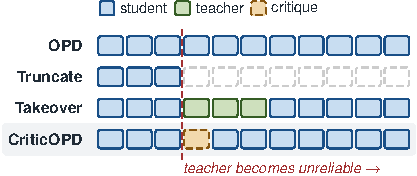
\includegraphics[width=\columnwidth]{figures/schematic.pdf}
%     \caption{Where the supervision of each method falls after the student errs, and who writes it.}
%     \label{fig:schematic}
% \end{figure}

% Prior work has found that this premise does not always hold, because the teacher completes the solution less reliably as the prefix of the student grows longer \citep{liu2026sfd, zhou2026early, li2026rethinking}. Existing methods respond in two ways (Figure~\ref{fig:schematic}). The first reduces supervision, which truncates the later part of long responses \citep{yang2026pruneopd, zhang2026fast} or stops rollouts or supervision early \citep{zhou2026early, liu2026prefix}. The second replaces the sequence, which lets the teacher take over a span of the generation \citep{xu2026pass, wang2026backtracking} or chooses between rollback and a teacher continuation \citep{jiang2026recoverability}. Both obtain reliable supervision by changing the sequence on which the student trains, and this change makes the mismatch between training and inference sequences larger than in standard OPD. Reducing supervision removes from training the later states that the student reaches at inference, and replacing the sequence trains the student on sequences that the teacher writes and the student would not generate. Both avoid the states where the teacher is unreliable instead of addressing this unreliability. In this work, we aim to keep the training sequences as close as possible to the inference sequences while keeping the supervision of the teacher on these sequences reliable.

% To measure reliability, we adopt recoverability from imitation learning \citep{swamy2021moments, jiang2026recoverability}, which we define as the accuracy of the teacher when it continues from a prefix of the student. This accuracy directly tests the premise above. We cut the rollouts of the student at several positions and let the teacher continue from each cut. On problems that the teacher solves readily, recoverability declines sharply along incorrect rollouts, and more than half of the supervision of the teacher on these rollouts falls on states from which it rarely continues correctly. The teacher fails at these states not because it cannot solve the problem but because it follows the errors of the student, and up to half of its failed continuations end with the incorrect answer of the student. Yet at these same states, the teacher still recognizes the errors of the student. After the student errs, the teacher thus loses the ability to continue correctly but keeps the ability to critique.

% Based on this observation, we propose CriticOPD, which uses the ability to critique that the teacher keeps to make its supervision reliable again after the student errs. Given the ground-truth answer, the teacher writes a critique of the incorrect solution of the student, which points out the errors and how to fix them. The student then rewrites its solution from the last error with the critique as a prompt. The teacher scores the rewrite with the critique in its context, while the student learns from the same sequence without the critique. The critique thus serves as privileged information \citep{vapnik2009lupi, lopezpaz2016unifying}, which the student sees only during training. This design keeps both properties (the last row of Figure~\ref{fig:schematic}). For the match, every token of the training sequence is still written by the student, and the critique only conditions the rewrite; we quantify the difference between the rewrite and the generation of the student without the critique in Section~\ref{sec:tradeoff}. For reliability, the teacher with the critique in its context can again rank a continuation that corrects the error above a continuation that extends it. Because the student learns without the critique, it must produce this correction by itself, which is the behavior that it needs at inference, where no critique is available.

% Our contributions are as follows:

% \begin{itemize}
%     \item We show that the supervision of OPD is no longer reliable after the student errs, because the teacher follows errors that it still recognizes, and that existing methods obtain reliable supervision at the cost of a larger mismatch between training and inference sequences.
%     \item We propose CriticOPD, which uses a critique that the teacher writes with the ground-truth answer as privileged information to make the supervision of the teacher reliable again, while every training sequence remains written by the student and the student trains without the critique.
%     \item We show, using two sizes of student model and six mathematical reasoning benchmarks, CriticOPD outperforms recent OPD variants obtaining reliable supervision with smaller mismatch. Our analysis shows that the critique sharpens the supervision signal toward the correction.
% \end{itemize}


% \begin{figure*}[t]
%     \centering
%     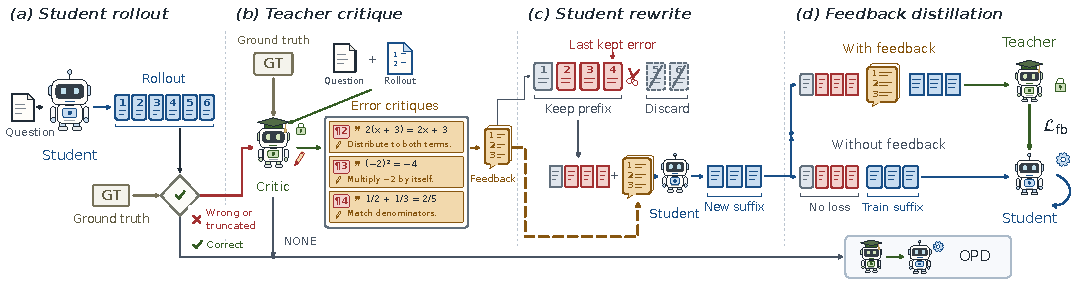
\includegraphics[width=\textwidth]{figures/fig_pipeline.pdf}
%     \caption{Overview of CriticOPD. The student rewrites an incorrect rollout from the last error that the teacher critiques. The teacher scores the rewrite with the critique, and the student learns from it without the critique.}
%     \label{fig:pipeline}
% \end{figure*}

\section{Introduction}
\label{sec:intro}


On-policy distillation (OPD) trains a student model on its own rollouts with token-level supervision from a teacher \citep{agarwal2024onpolicy, gu2023minillm}. OPD addresses a weakness of offline distillation. In offline distillation, the student trains on sequences the teacher generates, whereas the student at inference continues from prefixes that it generates itself, so the distribution of prefixes in training differs from the distribution of prefixes that the student visits at inference. We call the distance between these two distributions the occupancy mismatch. Under this mismatch, the errors of the student may be underrepresented in training, and once the student errs at inference, it may enter a prefix that it has rarely seen during training, allowing errors to accumulate \citep{ross2011dagger, agarwal2024onpolicy}. OPD reduces the occupancy mismatch by training on sequences that the student generates, with the next-token distribution of the teacher at each prefix as supervision. However, the effectiveness of this supervision in correcting errors depends on the teacher's ability to recover from the student's prefixes. When the teacher follows the student's errors rather than correcting them, its next-token distribution may no longer provide a reliable corrective target.


\begin{figure}[t]
    \centering
    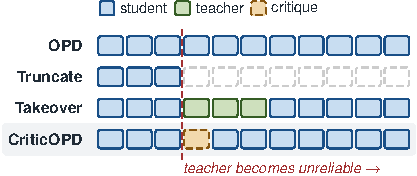
\includegraphics[width=\columnwidth]{figures/schematic.pdf}
    \caption{Where the supervision of each method falls after the student errs, and who writes it.}
    \label{fig:schematic}
\end{figure}


\begin{figure*}[t]
    \centering
    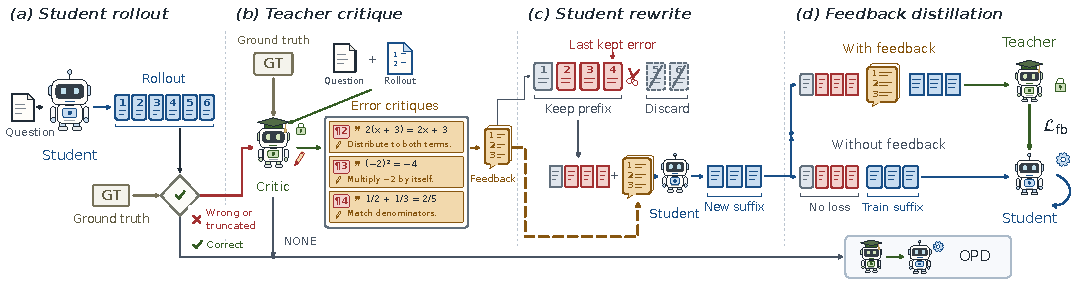
\includegraphics[width=\textwidth]{figures/fig_pipeline.pdf}
    \caption{Overview of CriticOPD. The student rewrites an incorrect rollout from the last error that the teacher critiques. The teacher scores the rewrite with the critique, and the student learns from it without the critique.}
    \label{fig:pipeline}
\end{figure*}

Prior work has found that teacher supervision can become less reliable as the prefix of the student grows longer \citep{liu2026sfd, zhou2026early, li2026rethinking}. Existing methods respond in two ways (Figure~\ref{fig:schematic}). The first reduces supervision. It truncates the later part of long responses \citep{yang2026pruneopd, zhang2026fast} or stops rollouts or supervision early \citep{zhou2026early, liu2026prefix}. The second replaces the sequence. It lets the teacher take over a span of
the generation \citep{xu2026relay} or regenerate from an earlier context
that the teacher judges reliable \citep{wang2026backtracking}. Both obtain more reliable supervision by restricting the states receiving supervision or modifying training trajectories, and thereby introduce more occupancy mismatch between training and inference than OPD. Reducing supervision leaves untrained the later states that the student reaches at inference, and replacing the sequence trains the student on sequences that the teacher writes and the student rarely generates. These methods largely avoid unreliable teacher supervision rather than improving its corrective value on erroneous student prefixes. In this work, we aim to make teacher supervision on student-generated continuations more reliable while introducing as little additional occupancy mismatch as possible.



We measure teacher reliability through recoverability, a notion from
imitation learning \citep{swamy2021moments}, which we define as the
teacher's accuracy when continuing from a student prefix. On incorrect rollouts, recoverability declines sharply even on problems the teacher can solve. The teacher often follows the student's errors, with up to half of its failed continuations ending in the student's incorrect answer. Yet its ability to identify errors remains largely intact. This reveals an asymmetry: the teacher may fail to continue correctly but still recognize errors.

Motivated by this observation, we propose CriticOPD. Given an incorrect rollout and the reference answer, the teacher identifies reasoning errors and provides corrective feedback. The student rewrites its solution from the last error using this feedback. The teacher then scores the rewrite with the critique in context, while the student learns without it. The critique serves as privileged information during training \citep{vapnik2009lupi,lopezpaz2016unifying}, enabling the student to learn corrective behavior without feedback at inference. Unlike teacher takeover, CriticOPD keeps all supervised tokens student-generated while improving the recoverability of the revised trajectories.



